\documentclass[]{book}
\usepackage{lmodern}
\usepackage{amssymb,amsmath}
\usepackage{ifxetex,ifluatex}
\usepackage{fixltx2e} % provides \textsubscript
\ifnum 0\ifxetex 1\fi\ifluatex 1\fi=0 % if pdftex
  \usepackage[T1]{fontenc}
  \usepackage[utf8]{inputenc}
\else % if luatex or xelatex
  \ifxetex
    \usepackage{mathspec}
  \else
    \usepackage{fontspec}
  \fi
  \defaultfontfeatures{Ligatures=TeX,Scale=MatchLowercase}
\fi
% use upquote if available, for straight quotes in verbatim environments
\IfFileExists{upquote.sty}{\usepackage{upquote}}{}
% use microtype if available
\IfFileExists{microtype.sty}{%
\usepackage{microtype}
\UseMicrotypeSet[protrusion]{basicmath} % disable protrusion for tt fonts
}{}
\usepackage[margin=1in]{geometry}
\usepackage{hyperref}
\hypersetup{unicode=true,
            pdftitle={Practical guide on dissolved organic matter (DOM) optic},
            pdfauthor={Philippe Massicotte},
            pdfborder={0 0 0},
            breaklinks=true}
\urlstyle{same}  % don't use monospace font for urls
\usepackage{natbib}
\bibliographystyle{apalike}
\usepackage{color}
\usepackage{fancyvrb}
\newcommand{\VerbBar}{|}
\newcommand{\VERB}{\Verb[commandchars=\\\{\}]}
\DefineVerbatimEnvironment{Highlighting}{Verbatim}{commandchars=\\\{\}}
% Add ',fontsize=\small' for more characters per line
\usepackage{framed}
\definecolor{shadecolor}{RGB}{248,248,248}
\newenvironment{Shaded}{\begin{snugshade}}{\end{snugshade}}
\newcommand{\KeywordTok}[1]{\textcolor[rgb]{0.13,0.29,0.53}{\textbf{{#1}}}}
\newcommand{\DataTypeTok}[1]{\textcolor[rgb]{0.13,0.29,0.53}{{#1}}}
\newcommand{\DecValTok}[1]{\textcolor[rgb]{0.00,0.00,0.81}{{#1}}}
\newcommand{\BaseNTok}[1]{\textcolor[rgb]{0.00,0.00,0.81}{{#1}}}
\newcommand{\FloatTok}[1]{\textcolor[rgb]{0.00,0.00,0.81}{{#1}}}
\newcommand{\ConstantTok}[1]{\textcolor[rgb]{0.00,0.00,0.00}{{#1}}}
\newcommand{\CharTok}[1]{\textcolor[rgb]{0.31,0.60,0.02}{{#1}}}
\newcommand{\SpecialCharTok}[1]{\textcolor[rgb]{0.00,0.00,0.00}{{#1}}}
\newcommand{\StringTok}[1]{\textcolor[rgb]{0.31,0.60,0.02}{{#1}}}
\newcommand{\VerbatimStringTok}[1]{\textcolor[rgb]{0.31,0.60,0.02}{{#1}}}
\newcommand{\SpecialStringTok}[1]{\textcolor[rgb]{0.31,0.60,0.02}{{#1}}}
\newcommand{\ImportTok}[1]{{#1}}
\newcommand{\CommentTok}[1]{\textcolor[rgb]{0.56,0.35,0.01}{\textit{{#1}}}}
\newcommand{\DocumentationTok}[1]{\textcolor[rgb]{0.56,0.35,0.01}{\textbf{\textit{{#1}}}}}
\newcommand{\AnnotationTok}[1]{\textcolor[rgb]{0.56,0.35,0.01}{\textbf{\textit{{#1}}}}}
\newcommand{\CommentVarTok}[1]{\textcolor[rgb]{0.56,0.35,0.01}{\textbf{\textit{{#1}}}}}
\newcommand{\OtherTok}[1]{\textcolor[rgb]{0.56,0.35,0.01}{{#1}}}
\newcommand{\FunctionTok}[1]{\textcolor[rgb]{0.00,0.00,0.00}{{#1}}}
\newcommand{\VariableTok}[1]{\textcolor[rgb]{0.00,0.00,0.00}{{#1}}}
\newcommand{\ControlFlowTok}[1]{\textcolor[rgb]{0.13,0.29,0.53}{\textbf{{#1}}}}
\newcommand{\OperatorTok}[1]{\textcolor[rgb]{0.81,0.36,0.00}{\textbf{{#1}}}}
\newcommand{\BuiltInTok}[1]{{#1}}
\newcommand{\ExtensionTok}[1]{{#1}}
\newcommand{\PreprocessorTok}[1]{\textcolor[rgb]{0.56,0.35,0.01}{\textit{{#1}}}}
\newcommand{\AttributeTok}[1]{\textcolor[rgb]{0.77,0.63,0.00}{{#1}}}
\newcommand{\RegionMarkerTok}[1]{{#1}}
\newcommand{\InformationTok}[1]{\textcolor[rgb]{0.56,0.35,0.01}{\textbf{\textit{{#1}}}}}
\newcommand{\WarningTok}[1]{\textcolor[rgb]{0.56,0.35,0.01}{\textbf{\textit{{#1}}}}}
\newcommand{\AlertTok}[1]{\textcolor[rgb]{0.94,0.16,0.16}{{#1}}}
\newcommand{\ErrorTok}[1]{\textcolor[rgb]{0.64,0.00,0.00}{\textbf{{#1}}}}
\newcommand{\NormalTok}[1]{{#1}}
\usepackage{longtable,booktabs}
\usepackage{graphicx,grffile}
\makeatletter
\def\maxwidth{\ifdim\Gin@nat@width>\linewidth\linewidth\else\Gin@nat@width\fi}
\def\maxheight{\ifdim\Gin@nat@height>\textheight\textheight\else\Gin@nat@height\fi}
\makeatother
% Scale images if necessary, so that they will not overflow the page
% margins by default, and it is still possible to overwrite the defaults
% using explicit options in \includegraphics[width, height, ...]{}
\setkeys{Gin}{width=\maxwidth,height=\maxheight,keepaspectratio}
\IfFileExists{parskip.sty}{%
\usepackage{parskip}
}{% else
\setlength{\parindent}{0pt}
\setlength{\parskip}{6pt plus 2pt minus 1pt}
}
\setlength{\emergencystretch}{3em}  % prevent overfull lines
\providecommand{\tightlist}{%
  \setlength{\itemsep}{0pt}\setlength{\parskip}{0pt}}
\setcounter{secnumdepth}{5}
% Redefines (sub)paragraphs to behave more like sections
\ifx\paragraph\undefined\else
\let\oldparagraph\paragraph
\renewcommand{\paragraph}[1]{\oldparagraph{#1}\mbox{}}
\fi
\ifx\subparagraph\undefined\else
\let\oldsubparagraph\subparagraph
\renewcommand{\subparagraph}[1]{\oldsubparagraph{#1}\mbox{}}
\fi

%%% Use protect on footnotes to avoid problems with footnotes in titles
\let\rmarkdownfootnote\footnote%
\def\footnote{\protect\rmarkdownfootnote}

%%% Change title format to be more compact
\usepackage{titling}

% Create subtitle command for use in maketitle
\newcommand{\subtitle}[1]{
  \posttitle{
    \begin{center}\large#1\end{center}
    }
}

\setlength{\droptitle}{-2em}
  \title{Practical guide on dissolved organic matter (DOM) optic}
  \pretitle{\vspace{\droptitle}\centering\huge}
  \posttitle{\par}
  \author{Philippe Massicotte}
  \preauthor{\centering\large\emph}
  \postauthor{\par}
  \predate{\centering\large\emph}
  \postdate{\par}
  \date{2016-09-01}


\begin{document}
\maketitle

{
\setcounter{tocdepth}{1}
\tableofcontents
}
\chapter{Introduction and
motivations}\label{introduction-and-motivations}

Dissolved organic matter (DOM) plays a central role in the functioning
of aquatic ecosystems. For example, characteristics of the DOM pool
(quantity and quality) determine underwater light climate
\citep{Kirk1994}, the composition of aquatic microbial communities
\citep{Foreman2003, Kritzberg2006a} and the carbon cycling on local to
global scales \citep{Cole2007}. Chemically, the DOM pool is complex
(\textgreater{} 1500 compounds) and analytical methods used to
characterize it are relatively complex, time-consuming and costly
\citep{Benner2002, Seitzinger2005, Fellman2010}. This situation called
for the development of rapid and cost effective characterization
techniques. Because optical properties of DOM can be related to its
chemical properties, optical techniques such as fluorescence
spectroscopy have been developed and rapidly adopted by the community to
characterize the DOM pool in aquatic ecosystems
\citep{Coble1990, Coble1996, McKnight2001}.

DOM is a complex mixture containing thousands of different chemical
compounds (ref). For this reasons, traditional chemical analysis used to
characterize DOM are both expensive and time consuming.

\begin{itemize}
\tightlist
\item
  Optical methods have been developed.
\item
  Why this project? Already few good books \citep{Lakowicz2006}
\item
  Need for unified way to present stuff with correct citation.
\item
  R code examples are also provided.
\item
  Wiki-like document that can serve as a starter for students.
\end{itemize}

\chapter{Measurements}\label{measurements}

\section{DOM measurements}\label{dom-measurements}

\begin{itemize}
\tightlist
\item
  How DOM is measured (different filter sizes, paper in L\&O).
\item
  Pump pression
\end{itemize}

\chapter{Absorbance}\label{absorbance}

\section{What is CDOM?}\label{what-is-cdom}

Chromophoric fraction of the DOM pool (CDOM) is a major driver of
underwater light characteristics (Kirk1994) which modulate many
bio-optical processes such as primary production (Thrane2014,
Seekell2015) and also constitute a natural screen protecting aquatic
organisms against harmful ultraviolet (UV) radiations (Boily2012).
Because of its colored nature, CDOM is known to strongly absorbs UV
light.

\citet{Blough2002} provide a good definition of what is CDOM.

\begin{quote}
Over the past decade, there has been a renewed interest in the
properties and distribution of the major light-absorbing constituent of
the (DOM) pool in natural waters (the 0.2 um fraction). This
material---referred in the past by various names such as Gelbstoff,
yellow substance, gilvin, and humic substances) has more recently been
provided the name chromophoric dissolved organic matter (CDOM).
\end{quote}

\begin{itemize}
\tightlist
\item
  Measured in quartz cuvette (1, 5, 10+ cm)
\end{itemize}

As wavelengths increase, light absorbed by CDOM decrease exponentially
\ref{fig:absorbance}.

\begin{Shaded}
\begin{Highlighting}[]
\KeywordTok{library}\NormalTok{(cdom)}
\KeywordTok{data}\NormalTok{(spectra)}

\NormalTok{spectra <-}\StringTok{ }\NormalTok{spectra %>%}\StringTok{ }\KeywordTok{filter}\NormalTok{(wavelength <=}\StringTok{ }\DecValTok{500}\NormalTok{)}

\NormalTok{p <-}\StringTok{ }\KeywordTok{ggplot}\NormalTok{(spectra, }\KeywordTok{aes}\NormalTok{(}\DataTypeTok{x =} \NormalTok{wavelength, }\DataTypeTok{y =} \NormalTok{spc1)) +}
\StringTok{  }\KeywordTok{geom_line}\NormalTok{() +}
\StringTok{  }\KeywordTok{xlab}\NormalTok{(}\StringTok{"Wavelength (nm.)"}\NormalTok{) +}
\StringTok{  }\KeywordTok{ylab}\NormalTok{(}\KeywordTok{bquote}\NormalTok{(Absorption~(nm^\{-}\DecValTok{1}\NormalTok{\})))}

\NormalTok{p}
\end{Highlighting}
\end{Shaded}

\begin{figure}[htbp]
\centering
\includegraphics{dom-optic_files/figure-latex/absorbance-1.pdf}
\caption{\label{fig:absorbance}Example of an absorption spectrum of CDOM.}
\end{figure}

\section{Writing and notation}\label{writing-and-notation}

In reference to this fraction of the DOM pool, people have been using
interchangeably different terminology. For example, a\_g(\(\lambda\)),
a(\(\lambda\)), CDOM(\(\lambda\)), aCDOM(\(\lambda\)) and
\(a_{CDOM}(\lambda)\) are all referring to the absorption coefficient
measured at wavelength \(\lambda\) (nm).

To unify the terminology, we propose that absorption of CDOM should be
written as \(\mathbf{a_{\text{CDOM}}(\lambda)}\) using the followings
\emph{rules}:

\begin{enumerate}
\def\labelenumi{\arabic{enumi}.}
\tightlist
\item
  \emph{a} in \emph{italic} to reference to absorption (vs absorbance).
\item
  CDOM subscripted and in capital letters.
\item
  \(\lambda\) sign to refer to the wavelength where the measurement is
  done.
\end{enumerate}

For example, \(a_{\text{CDOM}}(350)\) refers to absorption coefficient
measured at 350 nm.

\section{Absorption vs absorbance}\label{absorption-vs-absorbance}

\begin{equation}
a_{\text{CDOM}}(\lambda) = \frac{A(\lambda) \times 2.303}{L}
\label{eq:absorption}
\end{equation}

\section{Mathematical formulation of absorption
spectra}\label{mathematical-formulation-of-absorption-spectra}

As observed in figure \ref{fig:absorbance}, absorption decrease
exponentially with increasing wavelengths. \citet{Jerlov1968} and
\citet{Bricaud1981} first proposed to use a simple exponential
formulation to model absorption (equation \ref{eq:cdom1}).

\begin{equation}
a_{\text{CDOM}}(\lambda) = a_{\text{CDOM}}(\lambda0)e^{-S(\lambda - \lambda0)}
\label{eq:cdom1}
\end{equation}

Where \(a_{\text{CDOM}}(\lambda)\) is the absorption coefficient
(m\(^{-1}\)), \(\lambda\) is the wavelength (nm), \(\lambda0\) is a
reference wavelength (nm) and \(S\) is the spectral slope (nm\(^{-1}\))
that describes the approximate exponential rate of decrease of
absorption with increasing wavelength. Higher slopes indicate a more
rapid decrease in absorption with increasing wavelength. The \(S\)
parameter is frequently used as a proxy for tracing photochemical and
microbial-induced changes of CDOM
{[}Moran2000,Twardowski2004,Helms2013{]} or to determine its origin
{[}Stedmon2001{]}.

In 2001, equation \ref{eq:cdom1} was modified by \citet{Stedmon2001}
which introduced \(k\), a background constant (m\(^{-1}\)) accounting
for scatter in the cuvette and drift of the instrument (equation
\ref{eq:cdom2}).

\begin{equation}
a_{\text{CDOM}}(\lambda) = a_{\text{CDOM}}(\lambda0)e^{-S(\lambda - \lambda0)} + \mathbf{k}
\label{eq:cdom2}
\end{equation}

There are other mathematical formulations that can be used to model CDOM
spectra. These are reviewed in \citet{Twardowski2004}.

\section{Modeling CDOM absorption spectra in R}\label{sl}

Because of it inverse exponential shape, absorption spectra are best
modeled using non-linear fittings. In R this is done easy using the
\texttt{nls()} function. As we can see from equation \ref{eq:cdom2}, the
most commonly equation used to model CDOM spectra contains three
parameters: \texttt{a0,\ s,\ k}.

\begin{Shaded}
\begin{Highlighting}[]
\NormalTok{mod <-}\StringTok{ }\KeywordTok{nls}\NormalTok{(spc1 ~}\StringTok{ }\NormalTok{a0 *}\StringTok{ }\KeywordTok{exp}\NormalTok{(-s *}\StringTok{ }\NormalTok{(wavelength -}\StringTok{ }\DecValTok{250}\NormalTok{)) +}\StringTok{ }\NormalTok{k, }\CommentTok{# define the formula}
           \DataTypeTok{data =} \NormalTok{spectra, }\CommentTok{# where the data comes from}
           \DataTypeTok{start =} \KeywordTok{list}\NormalTok{(}\DataTypeTok{a0 =} \DecValTok{5}\NormalTok{, }\DataTypeTok{s =} \FloatTok{0.02}\NormalTok{, }\DataTypeTok{k =} \DecValTok{0}\NormalTok{)) }\CommentTok{# initial guesses.}

\CommentTok{# show the summary information}
\KeywordTok{summary}\NormalTok{(mod)}
\end{Highlighting}
\end{Shaded}

\begin{verbatim}
## 
## Formula: spc1 ~ a0 * exp(-s * (wavelength - 250)) + k
## 
## Parameters:
##     Estimate Std. Error t value Pr(>|t|)    
## a0 1.536e+01  4.778e-01   32.15   <2e-16 ***
## s  4.070e-02  5.989e-04   67.96   <2e-16 ***
## k  4.154e+00  2.871e-01   14.47   <2e-16 ***
## ---
## Signif. codes:  0 '***' 0.001 '**' 0.01 '*' 0.05 '.' 0.1 ' ' 1
## 
## Residual standard error: 4.187 on 308 degrees of freedom
## 
## Number of iterations to convergence: 7 
## Achieved convergence tolerance: 3.221e-06
\end{verbatim}

The value of \(a0\) is 15.36 represent the absorption coefficient at the
reference wavelength of 250 nm (Fig. \ref{fig:model}). The value of
\(S\) is 0.04 means that absorption is decreasing at a rate of 0.04
\(m^{-1}\) for each increase of 1 nm.

\begin{itemize}
\tightlist
\item
  k parameter (scattering, introduced by \citet{Stedmon2001})
\end{itemize}

\begin{Shaded}
\begin{Highlighting}[]
\NormalTok{p +}\StringTok{ }\KeywordTok{geom_line}\NormalTok{(}\KeywordTok{aes}\NormalTok{(}\DataTypeTok{y =} \KeywordTok{predict}\NormalTok{(mod)), }\DataTypeTok{col =} \StringTok{"red"}\NormalTok{) +}
\StringTok{  }\KeywordTok{geom_hline}\NormalTok{(}\DataTypeTok{yintercept =} \KeywordTok{coef}\NormalTok{(mod)[}\DecValTok{1}\NormalTok{] +}\StringTok{ }\KeywordTok{coef}\NormalTok{(mod)[}\DecValTok{3}\NormalTok{], }\DataTypeTok{lty =} \DecValTok{2}\NormalTok{) +}
\StringTok{  }\KeywordTok{geom_vline}\NormalTok{(}\DataTypeTok{xintercept =} \DecValTok{250}\NormalTok{, }\DataTypeTok{lty =} \DecValTok{2}\NormalTok{)}
\end{Highlighting}
\end{Shaded}

\begin{figure}[htbp]
\centering
\includegraphics{dom-optic_files/figure-latex/model-1.pdf}
\caption{\label{fig:model}Predicted values of the exponential model.}
\end{figure}

\subsection{Potential drawbacks}\label{potential-drawbacks}

When modeling CDOM spectra, there are few things to keep in minds that
can have a significant influence on model results.

\subsubsection{Choice of the reference
wavelength}\label{choice-of-the-reference-wavelength}

In equation \ref{eq:cdom2}, the reference wavelenght was set at 350 nm.
One question can potentially come to your mind. What is the effect of
choosing a different reference wavelengths? What will append to \(S\) if
we change the reference wavelength to let's say 250?

Fig. \ref{fig:refwl} shows that:

\begin{itemize}
\tightlist
\item
  Little effect (computational rounding)
\end{itemize}

\begin{figure}[htbp]
\centering
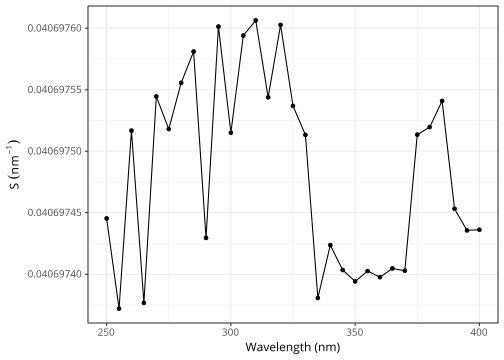
\includegraphics{dom-optic_files/figure-latex/refwl-1.pdf}
\caption{\label{fig:refwl}Effect of varying the reference wavelength on S.}
\end{figure}

\begin{itemize}
\tightlist
\item
  Plot the calculated curves on a graph
\end{itemize}

\subsubsection{Choice of the spectral
range}\label{choice-of-the-spectral-range}

\begin{itemize}
\tightlist
\item
  \citet{Massicotte2016MC}
\end{itemize}

\section{Metrics}\label{metrics}

\begin{itemize}
\tightlist
\item
  \(S_{300-600}\) linked to DOM molecular weight \citep{Stedmon2015b}.
\end{itemize}

\subsection{Slope ratio}\label{slope-ratio}

Equation \ref{eq:sr} shows how the slope ratio (\(S_R\)) is calculated.

\begin{equation}
S_R = \frac{S_{275-295}}{S_{350-400}}
\label{eq:sr}
\end{equation}

\begin{quote}
By calculating the ratio of the slope of the shorter wavelength region
(275--295 nm) to that of the longer wavelength region (350--400 nm), a
dimensionless parameter called ``slope ratio'' or \(S_R\) is defined.
This approach avoids the use of spectral data near the detection limit
of the instruments used, and focuses on absorbance values that shift
dramatically during estuarine transit and photochemical alteration of
CDOM \citep{Helms2008}.
\end{quote}

Figure \ref{fig:sr} shows in red the 275-295 and 350-400 nm spectral
range.

\begin{figure}[htbp]
\centering
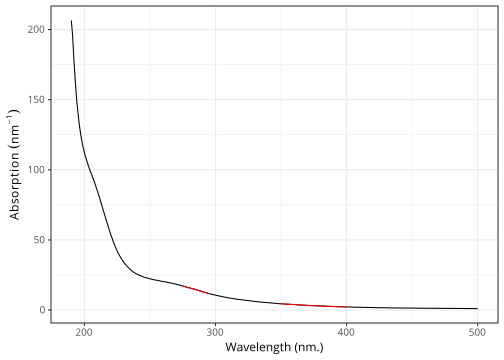
\includegraphics{dom-optic_files/figure-latex/sr-1.pdf}
\caption{\label{fig:sr}Spectral range used to calculate the slope ratio.}
\end{figure}

\chapter{Fluorescence}\label{fluorescence}

\section{What is a EEM}\label{what-is-a-eem}

\begin{figure}

{\centering \includegraphics{dom-optic_files/figure-latex/fig1-1} 

}

\caption{Example of an excitation-emission fluorescence matrix (EEM). The diagonal structure with high fluorescence corresponds to the first order of Rayleigh scattering.}\label{fig:fig1}
\end{figure}

\section{PARAFAC}\label{parafac}

The seminal paper of \citep{Stedmon2003a} put at the forefront the use
of parallel factor analysis (PARAFAC) to aid the characterization of
fluorescent DOM. Briefly, this three-way technique allows the
decomposition of complex DOM fluorescence signals contained in the
excitation-emission matrix (EEM, Fig. 1) into a set of individual
chemical components and provides estimations of their relative
contribution to the total fluorescence
\citep{Bro1997, Fellman2010, Stedmon2003a}.

The PARAFAC model is described as \citep{Bro1997, Harshman1970}:

\begin{equation}
x_{ijk} = \sum_{f=1}^{F} a_{ij}b_{jf}c_{kf} + e_{ijk}
\end{equation}

where \(i = 1, ..., I\); \(j = 1, ..., J\); \(k = 1, ..., K\),
\(x_{ijk}\) is the intensity of fluorescence of the the \(i^{th}\)
sample at the \(j^{th}\) emission wavelength at the \(k^{th}\)
excitation wavelength. \(a_{ij}\) is directly proportional to the
concentration of the \(f^{th}\) component in the sample \(i\). Although
PARAFAC gained a lot of attention in environmental sciences, it is also
widely used in other research fields such as medical, pharmaceutical,
food, social and information sciences \citep{Murphy2013}. Until today,
more than 1850 published scientific papers relying on PARAFAC have been
identified on Web of Science.

Although PARAFAC was made easier using the \texttt{drEEM} MATLAB toolbox
\citep{Murphy2013}, preprocessing of EEMs prior to the analysis is still
not straightforward. EEM preprocessing is an important part of PARAFAC
since it aims to correct any systematic bias in the measurements and to
remove signal unrelated to DOM fluorescence \citep{Murphy2013}. Biased
models can be produced if these steps are not conducted carefully (see
\citet{Hiriart-Baer2008} where scattering fluorescence signals have been
modeled and wrongly interpreted). Such data processing is cumbersome as
it involves many steps \citep{Stedmon2008, Murphy2013} which are usually
executed by hand or within in-house scripting and therefore prone to
introduce errors. Another important drawback limiting effective
preprocessing of EEMs arise from the wide variety of file formats
provided by the different manufacturers of spectrofluorometers that
makes data importation difficult to generalize.

Possibly reflecting these difficulties, it was recently pointed out that
characterization of DOM using fluorescence spectroscopy is still not
routinely included in ecological studies \citep{Fellman2010}. Given the
increasing interest for fluorescence spectroscopy in ecology, tools are
needed to unify the main preprocessing steps needed for further analyzes
such as PARAFAC or metric calculations. The purpose of the \texttt{eemR}
R package is to provide a rapid and an elegant interface to perform
preprocessing of EEMs as well as to extract common fluorescence-based
metrics proposed in the literature to obtain quantitative information
about the DOM pool. This paper presents theoretical and mathematical
background of the main PARAFAC preprocessing steps and metric
calculations with concrete code examples.

\section{Fluorescence of DOM: theoretical and mathematical
background}\label{fluorescence-of-dom-theoretical-and-mathematical-background}

Let us define \(X\), an EEM of fluorescence intensities measured along a
vector of excitation wavelengths (\(ex\)) at emission wavelengths
(\(em\)). Usually, \(ex\) and \(em\) vary, respectively, between 200-500
nm and 220-600 nm (Fig. 1). \(X_{ex, em}\) denotes the fluorescence
intensity measured at excitation \(ex\) and emission \(em\) (ex.:
\(X_{250, 400}\)).

The following sections present the main correction steps for
fluorescence data aiming to correct any systematic bias in the
measurements and remove signal unrelated to fluorescence prior to any
analysis.

\begin{longtable}[]{@{}lc@{}}
\toprule
\begin{minipage}[b]{0.25\columnwidth}\raggedright\strut
Correction\strut
\end{minipage} & \begin{minipage}[b]{0.46\columnwidth}\centering\strut
Description\strut
\end{minipage}\tabularnewline
\midrule
\endhead
\begin{minipage}[t]{0.25\columnwidth}\raggedright\strut
Blank subtraction\strut
\end{minipage} & \begin{minipage}[t]{0.46\columnwidth}\centering\strut
Subtract a pure water sample blank from the fluorescence data to help
the removal of Raman and Rayleigh scattering peaks.\strut
\end{minipage}\tabularnewline
\begin{minipage}[t]{0.25\columnwidth}\raggedright\strut
Scattering removal\strut
\end{minipage} & \begin{minipage}[t]{0.46\columnwidth}\centering\strut
Remove the the so-called scattering bands caused by first and second
order of Raman and Rayleigh scattering.\strut
\end{minipage}\tabularnewline
\begin{minipage}[t]{0.25\columnwidth}\raggedright\strut
Inner-filter effect correction\strut
\end{minipage} & \begin{minipage}[t]{0.46\columnwidth}\centering\strut
Correct for reabsorption of light occurring at both the excitation and
emission wavelengths during measurement.\strut
\end{minipage}\tabularnewline
\begin{minipage}[t]{0.25\columnwidth}\raggedright\strut
Raman normalization\strut
\end{minipage} & \begin{minipage}[t]{0.46\columnwidth}\centering\strut
Remove the dependency of fluorescence intensities from the measuring
equipments thus allowing cross-study comparisons.\strut
\end{minipage}\tabularnewline
\bottomrule
\end{longtable}

\subsection{Scattering correction}\label{scattering-correction}

Rayleigh and Raman scattering are optical processes by which some of the
incident energy can be absorbed and converted into vibrational and
rotational energy \citep{Lakowicz2006}. The resulting scattered energy
produce the so-called scattering bands which are visually easily
identifiable (Figs. 1 and 2). Given that both types of scattering are
repeated across EEMs, it is important to remove such artifacts prior to
analysis \citep{Bahram2006, Zepp2004}.

\begin{figure}

{\centering 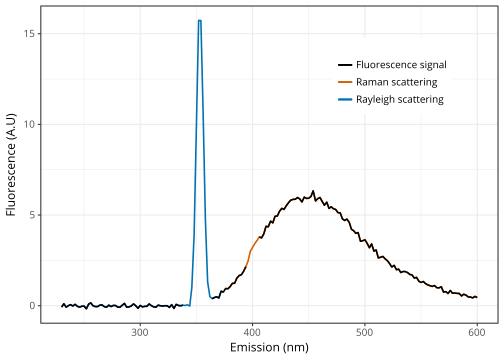
\includegraphics{dom-optic_files/figure-latex/fig2-1} 

}

\caption{Emission fluorescence emitted at excitation $ex = 350$. First order of Rayleigh and Raman scattering regions are identified in blue and red.}\label{fig:fig2}
\end{figure}

First order of Rayleigh scattering is defined as the region where
emission is equal to excitation (\(em = ex\)) causing a diagonal band in
the EEM (Fig. 1) whereas the second order of Rayleigh scattering occurs
at two times the emission wavelength of the primary peak (\(em = 2ex\)).
For water, Raman scattering occurs at a wavenumber 3 600 \(cm^{-1}\) (or
\(3.6 \times 10^{10} nm^{-1}\)) lower than the incident excitation
wavenumber \citep{Lakowicz2006}. Mathematically, first order Raman
scattering is defined as follow:

\begin{equation}
\text{Raman}_{\text{1st}} = -\frac{ex}{0.00036 ex - 1}
\label{eq:raman1}
\end{equation}

where \(ex\) is the incident excitation wavelength (nm). Second order
Raman scattering is then simply defined as:

\begin{equation}
\text{Raman}_{\text{2nd}} = -\frac{2ex}{0.00036 ex - 1}
\label{eq:raman2}
\end{equation}

Different interpolation techniques have been proposed to eliminate
scattering \citep{Zepp2004, Bahram2006}. However, it is a common
practice to simply remove the scattering-bands by inserting missing
values (Fig. 3) at the corresponding positions
\citep{Murphy2013, Stedmon2008}.

\subsection{Inner-filter effect
correction}\label{inner-filter-effect-correction}

The inner-filter effect (IFE) is an optical phenomenon of reabsorption
of emitted light and occurs particularly in highly concentrated samples
(Fig. 4). IFE is known to cause underestimation of fluorescence
intensities especially at shorter wavelengths and even to alter the
shape and the positioning of fluorescence spectra by shifting peak
positions toward lower wavelengths (Fig. 4) with increasing
concentration \citep{Mobed1996, Kothawala2013}. However, it was shown
that the loss of fluorescence due to IFE could be estimated from
absorbance spectra measured on the same sample using Equation
\ref{eq:ife} \citep{Ohno2002, Parker1957}:

\begin{equation}
X_0 = \frac{X}{10^{-b(A_{ex} + A_{em})}}
\label{eq:ife}
\end{equation}

where \(X_0\) is the fluorescence in the absence of IFE, \(X\) is the
measured fluorescence intensity, \(b\) is half the cuvette pathlength
(usually 0.5 cm) for excitation and emission absorbance, \(A_{ex}\) is
the absorbance at the excitation wavelength \(ex\) and \(A_{em}\) the
absorbance at the emission wavelength \(em\) (Fig. 4B).

It was recently shown that IFE corrected algebraically was not
appropriate when total absorbance, defined as
\(A_{\text{total}} = A_{\text{ex}} + A_{\text{em}}\) (see Equation
\ref{eq:ife}), is greater than 1.5 \citep{Kothawala2013}. Under this
circumstance, a two-fold dilution of the sample has been recommended. If
this happen, a warning message will be displayed by the package during
the correction process.

\subsection{Raman calibration}\label{raman-calibration}

The same DOM sample measured on different spectrofluorometers (or even
the same but with different settings) can give important differences in
fluorescence intensities \citep{Lawaetz2009, Coble1993}. The purpose of
the Raman calibration is to remove the dependency of fluorescence
intensities on the measuring equipment, thus allowing cross-study
comparisons. Given that the Raman peak position of a water sample is
located at a fixed position, \citep{Lawaetz2009} proposed to use the
Raman integral of a blank-water sample measured the same day as the EEM
to perform calibration. Moreover, the area of the Raman peak
(\(A_{\text{rp}}\), Fig. 5) is defined as the area of the emission
profile between 371 and 428 nm at a fixed excitation of 350 nm
\citep{Lawaetz2009}.

Mathematically, the value of \(A_{\text{rp}}\) is calculated using the
following integral (Equation\ref{eq:arp}):

\begin{equation}
A_{\text{rp}} = \int\limits_{\lambda_{\text{em}371}}^{\lambda_{\text{em}428}} W_{350, \lambda} d\lambda
\label{eq:arp}
\end{equation}

where \(W_{350, \lambda}\) is the fluorescence intensity of a pure water
sample (preferably deionized and ultraviolet exposed,
\citet{Lawaetz2009}) at excitation \(ex = 350\) nm and at emission
\(em = \lambda\) nm. Each values of the EEM \(X\) are then normalized
using the scalar value of \(A_{\text{rp}}\) accordingly to Equation
@ref(eq:raman\_normalisation):

\begin{equation}
X_0 = \frac{X}{A_{\text{rp}}}
\label{eq:raman_normalisation}
\end{equation}

where \(X_0\) is the normalized EEM with fluorescence intensities now
expressed as Raman Units (R.U.), \(X\) are the unnormalized measured
fluorescence intensities and \(A_{\text{rp}}\) is the Raman peak area.

\subsection{Metrics}\label{metrics-1}

A wide range of different metrics obtained from EEMs have been proposed
to characterize the DOM pool in aquatic ecosystems. These metrics
extract quantitative information in specific regions (wavelengths) in
EEMs. The following sections present an overview of the principal
metrics supported by the package.

\subsubsection{Coble's peaks}\label{cobles-peaks}

The following table presents the five major fluorescent components
identified by \citep{Coble1996} in marine EEMs. Peaks \textbf{B} and
\textbf{T} represent protein-like compounds (tyrosine and tryptophane),
peaks \textbf{A} and \textbf{C} are indicators of humic-like components
whereas peak \textbf{M} was associated to marine humic-like
fluorescence.

\begin{longtable}[]{@{}lll@{}}
\toprule
Peak & Ex (nm) & Em (nm)\tabularnewline
\midrule
\endhead
B & 275 & 310\tabularnewline
T & 275 & 340\tabularnewline
A & 260 & 380-460\tabularnewline
M & 312 & 380-420\tabularnewline
C & 350 & 420-480\tabularnewline
\bottomrule
\end{longtable}

\subsubsection{Fluorescence, humification and biological
indices}\label{fluorescence-humification-and-biological-indices}

Three main indices have been proposed to trace the diagnostic state of
the DOM pool in aquatic ecosystems. The fluorescence index (FI) was
shown to be a good indicator of the general source and aromaticity of
DOM in lakes, streams and rivers \citep{McKnight2001}. This index is
calculated as the ratio of fluorescence at emission 450 nm and 500 nm,
at fixed excitation of 370 nm (Equation \ref{eq:fi}).

\begin{equation}
\text{FI} = \frac{X_{370, 450}}{X_{370, 500}}
\label{eq:fi}
\end{equation}

The humification index (HIX) is a measure of the complexity and the
aromatic nature of DOM \citep{Ohno2002}. HIX calculated as the ratio of
the sum of the fluorescence between 435 and 480 nm and between 300 and
345 nm at a fixed excitation of 254 nm (Equation \ref{eq:hix}).

\begin{equation}
\text{HIX} = \frac{\sum\limits_{em = 435}^{480} X_{254, em}}{\sum\limits_{em = 300}^{345} X_{254, em}}
\label{eq:hix}
\end{equation}

The biological index (BIX) is a measure to characterize biological
production of DOM \citep{Huguet2009}. BIX is calculated at excitation
310 nm, by dividing the fluorescence intensity emitted at emission 380
nm and at 430 nm (Equation (\ref{eq:bix})).

\begin{equation}
\text{BIX} = \frac{X_{310, 380}}{X_{310, 430}}
\label{eq:bix}
\end{equation}

\section{R code and study case}\label{r-code-and-study-case}

Main preprocessing steps using the \textbf{eemR} package are illustrated
using a subset of three EEMs from \citep{Massicotte2011EA}. Briefly,
these EEMs (see Fig. 1 for an example) have been sampled in the
St.~Lawrence River, one of the largest rivers in North America.
Fluorescence matrices of DOM were measured on a Cary Eclipse
spectrofluorometer (Varian, Mississauga, Ontario, Canada) over
excitation wavelengths between 220 and 450 nm (5-nm increment) and
emission wavelengths between 230 and 600 nm (2-nm increment). All
functions from the package start with the prefix
\texttt{\textquotesingle{}eem\_\textquotesingle{}}.

\begin{Shaded}
\begin{Highlighting}[]
\KeywordTok{library}\NormalTok{(eemR)}
\KeywordTok{ls}\NormalTok{(}\StringTok{"package:eemR"}\NormalTok{)}
\end{Highlighting}
\end{Shaded}

\begin{verbatim}
##  [1] "absorbance"              "eem_bind"               
##  [3] "eem_biological_index"    "eem_coble_peaks"        
##  [5] "eem_cut"                 "eem_export_matlab"      
##  [7] "eem_extract"             "eem_fluorescence_index" 
##  [9] "eem_humification_index"  "eem_inner_filter_effect"
## [11] "eem_names"               "eem_names<-"            
## [13] "eem_raman_normalisation" "eem_read"               
## [15] "eem_read_parafac"        "eem_remove_blank"       
## [17] "eem_remove_scattering"   "eem_set_wavelengths"
\end{verbatim}

\subsection{Data importation and
plotting}\label{data-importation-and-plotting}

Importation of EEMs into R is done using the \texttt{eem\_read()}
function. Given that fluorescence files are dependent on the
spectrofluorometer used, \texttt{eemR} will determine automatically from
which manufacturer the files are from and load them accordingly.

\begin{Shaded}
\begin{Highlighting}[]
\NormalTok{file <-}\StringTok{ }\KeywordTok{system.file}\NormalTok{(}\StringTok{"extdata/cary/scans_day_1"}\NormalTok{, }\DataTypeTok{package =} \StringTok{"eemR"}\NormalTok{)}
\NormalTok{eems <-}\StringTok{ }\KeywordTok{eem_read}\NormalTok{(file)}
\end{Highlighting}
\end{Shaded}

The generic \texttt{summary()} function displays useful information such
as: (1) the wavelength ranges used in both emission and excitation
modes, (2) the manufacturer from which the file was read and (3) the
state of the EEM which indicate which corrections have been applied.

\begin{Shaded}
\begin{Highlighting}[]
\KeywordTok{summary}\NormalTok{(eems)}
\end{Highlighting}
\end{Shaded}

\begin{verbatim}
##    sample ex_min ex_max em_min em_max is_blank_corrected
## 1    nano    220    450    230    600              FALSE
## 2 sample1    220    450    230    600              FALSE
## 3 sample2    220    450    230    600              FALSE
## 4 sample3    220    450    230    600              FALSE
##   is_scatter_corrected is_ife_corrected is_raman_normalized manufacturer
## 1                FALSE            FALSE               FALSE Cary Eclipse
## 2                FALSE            FALSE               FALSE Cary Eclipse
## 3                FALSE            FALSE               FALSE Cary Eclipse
## 4                FALSE            FALSE               FALSE Cary Eclipse
\end{verbatim}

A surface plot of EEMs is made using the \texttt{plot(x,\ which\ =\ 1)}
function where \texttt{which} is the index of the EEM to be plotted (see
Fig. 3).

\begin{Shaded}
\begin{Highlighting}[]
\KeywordTok{plot}\NormalTok{(eems, }\DataTypeTok{which =} \DecValTok{3}\NormalTok{)}
\end{Highlighting}
\end{Shaded}

Interactive plots using a simple shiny app can be lunched to
interactively browse EEMs.

\begin{Shaded}
\begin{Highlighting}[]
\KeywordTok{plot}\NormalTok{(eems, }\DataTypeTok{interactive =} \OtherTok{TRUE}\NormalTok{)}
\end{Highlighting}
\end{Shaded}

\subsection{Blank subtraction}\label{blank-subtraction}

Subtraction of a water blank from the measured samples may help to
reduce scattering \citep{Murphy2013, Stedmon2008}. In \texttt{eemR},
this is done using the \texttt{eem\_remove\_blank(eem,\ blank)} function
where \texttt{eem} is a list of EEMs and \texttt{blank} is a water
blank.

\begin{Shaded}
\begin{Highlighting}[]
\NormalTok{file <-}\StringTok{ }\KeywordTok{system.file}\NormalTok{(}\StringTok{"extdata/cary/scans_day_1"}\NormalTok{, }\StringTok{"nano.csv"}\NormalTok{, }\DataTypeTok{package =} \StringTok{"eemR"}\NormalTok{)}
\NormalTok{blank <-}\StringTok{ }\KeywordTok{eem_read}\NormalTok{(file)}

\NormalTok{eems <-}\StringTok{ }\KeywordTok{eem_remove_blank}\NormalTok{(eems, blank)}
\end{Highlighting}
\end{Shaded}

\subsection{Raman and Rayleigh scattering
removal}\label{raman-and-rayleigh-scattering-removal}

Scattering removal (Equation \ref{eq:raman1} and Equation
\ref{eq:raman2}) is performed using the
\texttt{eem\_remove\_scattering(eem,\ type,\ order,\ width)} function
where \texttt{eem} is a list of EEMs, \texttt{type} is the scattering
type (\texttt{raman} or \texttt{rayleigh}), \texttt{order} is the order
of the scattering (1 or 2) and \texttt{width} the width in nanometers of
the slit windows to be removed. In the following example, only first
order and Raman and Rayleigh scattering are removed using a bandwidth of
10 nm (Fig. 3).

\begin{Shaded}
\begin{Highlighting}[]
\NormalTok{eems <-}\StringTok{ }\KeywordTok{eem_remove_scattering}\NormalTok{(eems, }\StringTok{"rayleigh"}\NormalTok{, }\DecValTok{1}\NormalTok{, }\DecValTok{10}\NormalTok{) %>%}
\StringTok{  }\KeywordTok{eem_remove_scattering}\NormalTok{(}\StringTok{"raman"}\NormalTok{, }\DecValTok{1}\NormalTok{, }\DecValTok{10}\NormalTok{)}

\KeywordTok{plot}\NormalTok{(eems, }\DataTypeTok{which =} \DecValTok{3}\NormalTok{)}
\end{Highlighting}
\end{Shaded}

\begin{figure}

{\centering \includegraphics{dom-optic_files/figure-latex/fig5-1} 

}

\caption{Fluorescence profile of a pure water sample at excitation 350 nm between 300 and 450 nm emission. The area of the Raman peak is identified by the shaded polygon and is calculated using Equation xxx.}\label{fig:fig5}
\end{figure}

\subsection{Inner-filter effect
correction}\label{inner-filter-effect-correction-1}

IFE correction requires the use of absorbance data (Equation
\ref{eq:ife}). For each EEM, an absorbance spectra must be supplied. The
easiest way to provide absorbance is to use a data frame with column
names matching EEMs names. In the following data frame, the first column
represents the wavelengths at which absorbance have been measured
whereas the remaining columns are absorbance spectra for
\texttt{sample1}, \texttt{sample2} and \texttt{sample3}.

\begin{Shaded}
\begin{Highlighting}[]
\KeywordTok{data}\NormalTok{(}\StringTok{"absorbance"}\NormalTok{)}
\KeywordTok{head}\NormalTok{(absorbance)}
\end{Highlighting}
\end{Shaded}

\begin{verbatim}
##   wavelength sample1 sample2 sample3
## 1        190 0.89674 1.02927 1.19405
## 2        191 0.84894 0.96381 1.13721
## 3        192 0.77267 0.85339 1.04520
## 4        193 0.70967 0.75627 0.96782
## 5        194 0.65459 0.67145 0.90092
## 6        195 0.61371 0.60745 0.85054
\end{verbatim}

Note that EEM names can be obtained using the
\texttt{eem\_sample\_names()} function.

\begin{Shaded}
\begin{Highlighting}[]
\KeywordTok{eem_names}\NormalTok{(eems)}
\end{Highlighting}
\end{Shaded}

\begin{verbatim}
## [1] "nano"    "sample1" "sample2" "sample3"
\end{verbatim}

IFE correction is performed using the
\texttt{eem\_inner\_filter\_effect(eem,\ absorbance,\ pathlength)}
function where \texttt{eem} is a list of EEMs, \texttt{absorbance} is a
data frame containing absorbance spectra and \texttt{pathlength} is the
absorbance cuvette pathlength expressed in \(cm\) (Fig. 4B). For each
EEM contained in \texttt{eem}, the ranges spanned by the IFE correction
factors and total absorbance \(A_{\text{total}}\) (Equation
\ref{eq:ife}) are displayed to the user. This can serve as diagnostic
tool to determine if the mathematical correction was the appropriate
method to use to handle IFE.

\begin{Shaded}
\begin{Highlighting}[]
\NormalTok{eems <-}\StringTok{ }\KeywordTok{eem_inner_filter_effect}\NormalTok{(}\DataTypeTok{eem =} \NormalTok{eems,}
                                \DataTypeTok{absorbance =} \NormalTok{absorbance,}
                                \DataTypeTok{pathlength =} \DecValTok{1}\NormalTok{)}
\end{Highlighting}
\end{Shaded}

\begin{verbatim}
## Warning: Absorbance spectrum for nano was not found. Returning uncorrected
## EEM.
\end{verbatim}

\begin{verbatim}
## Range of IFE correction factors: 0.6433 0.989 
## Range of total absorbance (Atotal) : 0.0096 0.3832 
## Range of IFE correction factors: 0.7619 0.994 
## Range of total absorbance (Atotal) : 0.0053 0.2362 
## Range of IFE correction factors: 0.4217 0.9843 
## Range of total absorbance (Atotal) : 0.0138 0.75
\end{verbatim}

\begin{Shaded}
\begin{Highlighting}[]
\KeywordTok{plot}\NormalTok{(eems, }\DataTypeTok{which =} \DecValTok{3}\NormalTok{)}
\end{Highlighting}
\end{Shaded}

Fig. 4 presents intermediate results obtained for the correction of
\texttt{sample3}. Note the nonlinearity of the correction with higher
effect at lower wavelengths (bottom-left corner in panel C). The
corrected EEM is presented in Fig. 4D which is the result of the
operation of dividing matrix in 4A by 4C.

\subsection{Raman normalization}\label{raman-normalization}

The last step of the correction process consist to calibrate
fluorescence intensities using the Raman scatter peak of water
\citep{Lawaetz2009}. This is performed using the
\texttt{eem\_raman\_normalisation(eem,\ blank)} function where
\texttt{eem} is a list of EEMs and \texttt{blank} is a water blank
measured the same day. Here, the same water-blank is used for the three
EEMs. Note that the value of the Raman area (\(A_{\text{rp}}\),
Equation\ref{eq:arp}) is printed.

\begin{Shaded}
\begin{Highlighting}[]
\NormalTok{eems <-}\StringTok{ }\KeywordTok{eem_raman_normalisation}\NormalTok{(eems, blank)}
\end{Highlighting}
\end{Shaded}

\begin{verbatim}
## Raman area: 9.540904 
## Raman area: 9.540904 
## Raman area: 9.540904
\end{verbatim}

\begin{Shaded}
\begin{Highlighting}[]
\KeywordTok{plot}\NormalTok{(eems, }\DataTypeTok{which =} \DecValTok{3}\NormalTok{)}
\end{Highlighting}
\end{Shaded}

At this stage, all corrections have been performed and EEMs are ready to
be exported into MATLAB for PARAFAC analysis. The state of the EEMs can
be verified using the \texttt{summary()} function.

\begin{Shaded}
\begin{Highlighting}[]
\KeywordTok{summary}\NormalTok{(eems)}
\end{Highlighting}
\end{Shaded}

\begin{verbatim}
##    sample ex_min ex_max em_min em_max is_blank_corrected
## 1    nano    220    450    230    600              FALSE
## 2 sample1    220    450    230    600               TRUE
## 3 sample2    220    450    230    600               TRUE
## 4 sample3    220    450    230    600               TRUE
##   is_scatter_corrected is_ife_corrected is_raman_normalized manufacturer
## 1                 TRUE            FALSE               FALSE Cary Eclipse
## 2                 TRUE             TRUE                TRUE Cary Eclipse
## 3                 TRUE             TRUE                TRUE Cary Eclipse
## 4                 TRUE             TRUE                TRUE Cary Eclipse
\end{verbatim}

\subsection{Exporting to MATLAB}\label{exporting-to-matlab}

The \textbf{drEEM} MATLAB toolbox \citep{Murphy2013} used to perform
PARAFAC analysis requires data in a specific format (structure). The
\texttt{eem\_export\_matlab(file,\ ...)} function can be used to export
corrected EEMs into a PARAFAC ready format. The first \texttt{file}
argument is the mat file where to export the structure and the second
argument \texttt{...} is one or more \texttt{eem} object.

\begin{Shaded}
\begin{Highlighting}[]
\KeywordTok{eem_export_matlab}\NormalTok{(}\StringTok{"myfile.mat"}\NormalTok{, eems)}
\end{Highlighting}
\end{Shaded}

Once exported, one can simply import the generated mat file in MATLAB
using \texttt{load(\textquotesingle{}myfile.mat\textquotesingle{});}.

\subsection{Metric extraction}\label{metric-extraction}

Coble's peaks can be extracted using the \texttt{eem\_coble\_peaks(eem)}
function. Note that for peaks \textbf{A, M, C}, the maximum fluorescence
intensity in the range of emission region is returned.

\begin{Shaded}
\begin{Highlighting}[]
\NormalTok{file <-}\StringTok{ }\KeywordTok{system.file}\NormalTok{(}\StringTok{"extdata/cary/scans_day_1"}\NormalTok{, }\DataTypeTok{package =} \StringTok{"eemR"}\NormalTok{)}
\NormalTok{eems <-}\StringTok{ }\KeywordTok{eem_read}\NormalTok{(file)}

\KeywordTok{eem_coble_peaks}\NormalTok{(eems, }\DataTypeTok{verbose =} \OtherTok{FALSE}\NormalTok{)}
\end{Highlighting}
\end{Shaded}

\begin{verbatim}
##    sample         b         t        a          m         c
## 1    nano 0.8745673 0.1401188 0.140175 0.09653326 0.1255788
## 2 sample1 1.5452981 1.0603312 3.731836 2.42409567 1.8149415
## 3 sample2 1.2629968 0.6647042 1.583489 1.02359302 0.7709074
## 4 sample3 1.4740862 1.3162812 8.416034 6.06335506 6.3179129
\end{verbatim}

Fluorescence (FI), humification (HIX) and biological (BIX) indices can
be extracted as follow.

\begin{Shaded}
\begin{Highlighting}[]
\KeywordTok{eem_fluorescence_index}\NormalTok{(eems, }\DataTypeTok{verbose =} \OtherTok{FALSE}\NormalTok{)}
\end{Highlighting}
\end{Shaded}

\begin{verbatim}
##    sample         fi
## 1    nano -0.5932057
## 2 sample1  1.2647823
## 3 sample2  1.4553330
## 4 sample3  1.3294132
\end{verbatim}

\begin{Shaded}
\begin{Highlighting}[]
\KeywordTok{eem_humification_index}\NormalTok{(eems, }\DataTypeTok{verbose =} \OtherTok{FALSE}\NormalTok{)}
\end{Highlighting}
\end{Shaded}

\begin{verbatim}
##    sample        hix
## 1    nano  0.5568136
## 2 sample1  6.3795618
## 3 sample2  4.2548483
## 4 sample3 13.0246234
\end{verbatim}

\begin{Shaded}
\begin{Highlighting}[]
\KeywordTok{eem_biological_index}\NormalTok{(eems, }\DataTypeTok{verbose =} \OtherTok{FALSE}\NormalTok{)}
\end{Highlighting}
\end{Shaded}

\begin{verbatim}
##    sample       bix
## 1    nano 2.6812045
## 2 sample1 0.7062640
## 3 sample2 0.8535423
## 4 sample3 0.4867927
\end{verbatim}

It should be noted that different excitation and emission wavelengths
are often used to measure EEMs. Hence, it is possible to have mismatch
between measured wavelengths and wavelengths used to calculate specific
metrics. In these circumstances, EEMs are interpolated using the the
\texttt{pracma} package \citep{Borchers2015}. A message warning the user
will be displayed if data interpolation is performed. This behavior can
be controlled using the \texttt{verbose\ =\ TRUE/FALSE} parameter.

\section{Using R pipeline}\label{using-r-pipeline}

Note that it is also possible to use the
\href{https://cran.r-project.org/web/packages/magrittr/vignettes/magrittr.html}{magrittr}
pipe line with most functions from \texttt{eemR}.

\begin{Shaded}
\begin{Highlighting}[]
\KeywordTok{library}\NormalTok{(magrittr)}

\NormalTok{file <-}\StringTok{ }\KeywordTok{system.file}\NormalTok{(}\StringTok{"extdata/cary/scans_day_1/"}\NormalTok{, }\DataTypeTok{package =} \StringTok{"eemR"}\NormalTok{)}
\NormalTok{file %>%}
\StringTok{  }\KeywordTok{eem_read}\NormalTok{(}\DataTypeTok{recursive =} \OtherTok{TRUE}\NormalTok{) %>%}
\StringTok{  }\KeywordTok{eem_raman_normalisation}\NormalTok{() %>%}
\StringTok{  }\KeywordTok{eem_remove_scattering}\NormalTok{(}\DataTypeTok{type =} \StringTok{"raman"}\NormalTok{, }\DataTypeTok{order =} \DecValTok{1}\NormalTok{, }\DataTypeTok{width =} \DecValTok{10}\NormalTok{) %>%}
\StringTok{  }\KeywordTok{eem_remove_scattering}\NormalTok{(}\DataTypeTok{type =} \StringTok{"rayleigh"}\NormalTok{, }\DataTypeTok{order =} \DecValTok{1}\NormalTok{, }\DataTypeTok{width =} \DecValTok{10}\NormalTok{) %>%}
\StringTok{  }\KeywordTok{plot}\NormalTok{(}\DecValTok{2}\NormalTok{)}
\end{Highlighting}
\end{Shaded}

\bibliography{/home/persican/Documents/library.bib}


\end{document}
